\documentclass[11pt,table]{beamer}
\mode<presentation>
\usepackage{etex}
\usepackage{graphicx}
\usepackage{epstopdf}
\usepackage[english]{babel}
\usepackage{tabularx}
\usepackage{booktabs}
\usepackage{mathrsfs}
\usepackage{multicol}
\usepackage{bm}
\usepackage{subcaption}
\usepackage{wrapfig}
\usepackage{dcolumn}
\usepackage{threeparttable}
\usepackage{booktabs}
\usepackage{bbm}
\usepackage{amsmath,dsfont,listings}
\usepackage{amssymb}
\usepackage{rotating}
\usepackage{multirow}
\usepackage[authoryear]{natbib}
\usepackage{circledsteps}
\usepackage{tikz}
\usetikzlibrary{arrows,decorations.pathmorphing,backgrounds,fit,positioning,shapes.symbols,chains}
\setbeamertemplate{section in toc}[sections numbered]
\setbeamertemplate{caption}[numbered]

\bibliographystyle{Econometrica}

\setbeamersize{text margin right=3.5mm, text margin left=7.5mm}  % text margin
\setbeamersize{sidebar width left=0cm, sidebar width right=0mm}
\setbeamertemplate{sidebar right}{}
\setbeamertemplate{sidebar left}{}

\definecolor{text-grey}{rgb}{0.45, 0.45, 0.45} % grey text on white background
\definecolor{bg-grey}{rgb}{0.66, 0.65, 0.60} % grey background (for white text)
\definecolor{fu-blue}{RGB}{0, 51, 102} % blue text
\definecolor{fu-green}{RGB}{153, 204, 0} % green text
\definecolor{fu-red}{RGB}{204, 0, 0} % red text (used by \alert)

\setbeamertemplate{frametitle}{%
    \vskip-30pt \color{text-grey}\large%
    \begin{minipage}[b][23pt]{80.5mm}%
    \flushleft\insertframetitle%
    \end{minipage}%
}

\setbeamertemplate{navigation symbols}{} 

%%% begin title page
\setbeamertemplate{title page}{
\vskip2pt\hfill
\vskip6pt\hskip3pt

% set the title and the author
\vskip14pt
\parbox[top][1.35cm][c]{11cm}{\LARGE\color{text-grey}\inserttitle \\[1ex] \small \insertsubtitle \\[3ex]}
\vskip11pt
\parbox[top][1.35cm][c]{11cm}{\small \insertauthor \; \insertinstitute \\[2ex] \insertdate}
}
%%% end title page

%%% colors
\usecolortheme{lily}
\setbeamercolor*{normal text}{fg=black,bg=white}
\setbeamercolor*{alerted text}{fg=fu-red}
\setbeamercolor*{example text}{fg=fu-green}
\setbeamercolor*{structure}{fg=fu-blue}

\setbeamercolor*{block title}{fg=white,bg=black!50}
\setbeamercolor*{block title alerted}{fg=white,bg=black!50}
\setbeamercolor*{block title example}{fg=white,bg=black!50}

\setbeamercolor*{block body}{bg=black!10}
\setbeamercolor*{block body alerted}{bg=black!10}
\setbeamercolor*{block body example}{bg=black!10}

\setbeamercolor{bibliography entry author}{fg=fu-blue}
\setbeamercolor{bibliography entry journal}{fg=text-grey}
\setbeamercolor{item}{fg=fu-blue}
\setbeamercolor{navigation symbols}{fg=text-grey,bg=bg-grey}
%%% end colors

%%% headline
\setbeamertemplate{headline}{
\vskip30pt
}
%%% end headline

%%% footline
\newcommand{\footlinetext}{
%\insertshortinstitute, \insertshorttitle, \insertshortdate
}
\setbeamertemplate{footline}{
\vskip2pt
\hfill \raisebox{-1pt}{\usebeamertemplate***{navigation symbols}}
\hfill \insertframenumber\hspace{10pt}
\vskip4pt
}
%%% end footline

%%% settings for listings package
\lstset{extendedchars=true, showstringspaces=false, basicstyle=\footnotesize\sffamily, tabsize=2, breaklines=true, breakindent=10pt, frame=l, columns=fullflexible}
\lstset{language=Java} % this sets the syntax highlighting
\lstset{mathescape=true} % this switches on $...$ substitution in code
% enables UTF-8 in source code:
\lstset{literate={�}{{\"a}}1 {�}{{\"o}}1 {�}{{\"u}}1 {�}{{\"A}}1 {�}{{\"O}}1 {�}{{\"U}}1 {�}{\ss}1}
%%% end listings

\usepackage{concmath}
\usepackage{xcolor}
\definecolor{red1}{RGB}{206, 17, 38}
\definecolor{blue1}{RGB}{16, 118, 208}
\definecolor{gray1}{RGB}{117, 115, 115}
\usepackage{hyperref}
\hypersetup{
    bookmarks=false,
    unicode=false,
    pdftoolbar=false,
    pdffitwindow=true,
    pdftitle={Econometricks: Short guides to econometrics},
    pdfauthor={Davud Rostam-Afschar},
    pdfsubject={econometrics},
    pdfcreator={Davud Rostam-Afschar},
    pdfproducer={Davud Rostam-Afschar},
    pdfkeywords={econometrics},
    pdfnewwindow=true,
}

\newtheorem{proposition}{Proposition}
\newtheorem{assumption}{Definition}


\title[] 
{Econome\textcolor{red1}{tricks}: Short guides to econometrics\\[1ex]\normalsize 
}

\author[D. Rostam-Afschar]{Trick 02: Specific Distributions\\[2ex]}

\institute[]{\textcolor{gray1}{Davud Rostam-Afschar (Uni Mannheim)}}
            
\date[] 
{}

\subject{Econometrics}
\renewcommand{\footlinetext}{\insertshortinstitute, \insertshorttitle, \insertshortdate}

\def\sym#1{\ifmmode^{#1}\else\(^{#1}\)\fi}

\begin{document}

\begin{frame}[plain]
  \titlepage
\end{frame}

% --------------------------------------------------- Slide --
\begin{frame}
	\frametitle{Content}
	\tableofcontents[]
\end{frame}



\begin{frame}{Specific Distributions}
\begin{figure}[H]
\begin{center}
{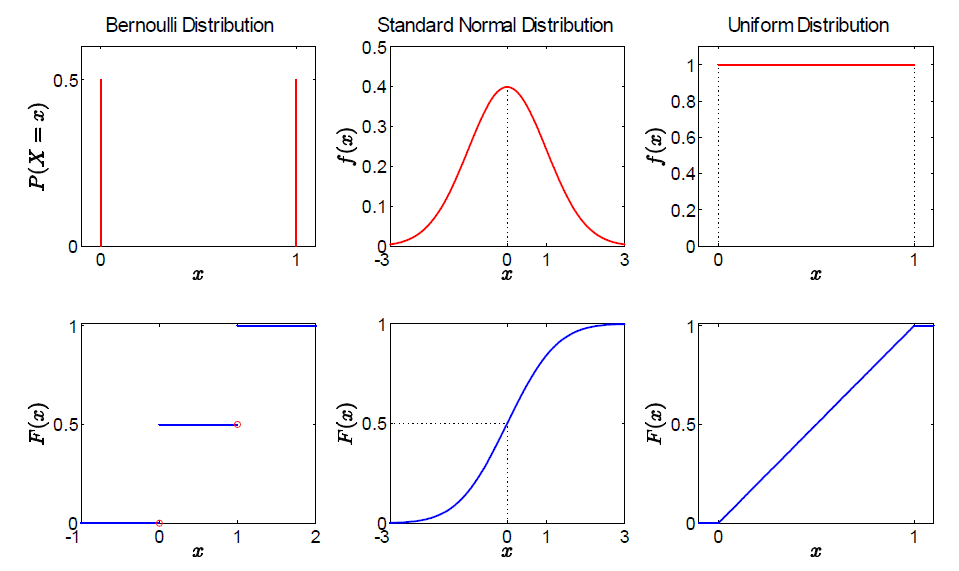
\includegraphics[width=0.8\textwidth]{figures/distributions}}\label{f1}
\end{center}
\end{figure}
\tiny Thanks to Ping Yu
\end{frame}


\begin{frame}{Discrete distributions}
The $\textbf{Bernoulli distribution}$ for a single binomial outcome (trial) is
\begin{eqnarray*}
  Prob(x = 1) &=& p, \\
  Prob(x = 0) &=& 1-p,
\end{eqnarray*}
where $0 \leq p \leq 1$ is the probability of success.

\begin{itemize}
	\item  $E[x]=p$ and 
	\item $V[x]=E[x^2]-E[x]^2=p-p^2=p(1-p)$.
\end{itemize}
 

\end{frame}

\begin{frame}{Discrete distributions}
 The distribution for $x$ successes in $n$ trials is the $\textbf{binomial distribution}$,
\begin{equation*}
    Prob(X = x) =\frac{n!}{(n-x)!x!}p^{x}(1-p)^{n-x}~~~x =0, 1,\ldots, n.
\end{equation*}
The mean and variance of $x$ are
\begin{itemize}
	\item  $E[x]=np$ and 
	\item $V[x]=np(1 - p)$.
\end{itemize}

Example of a binomial $[n=15,p=0.5]$ distribution:

\begin{figure}[H]
\begin{center}
%\scalebox{.36}
{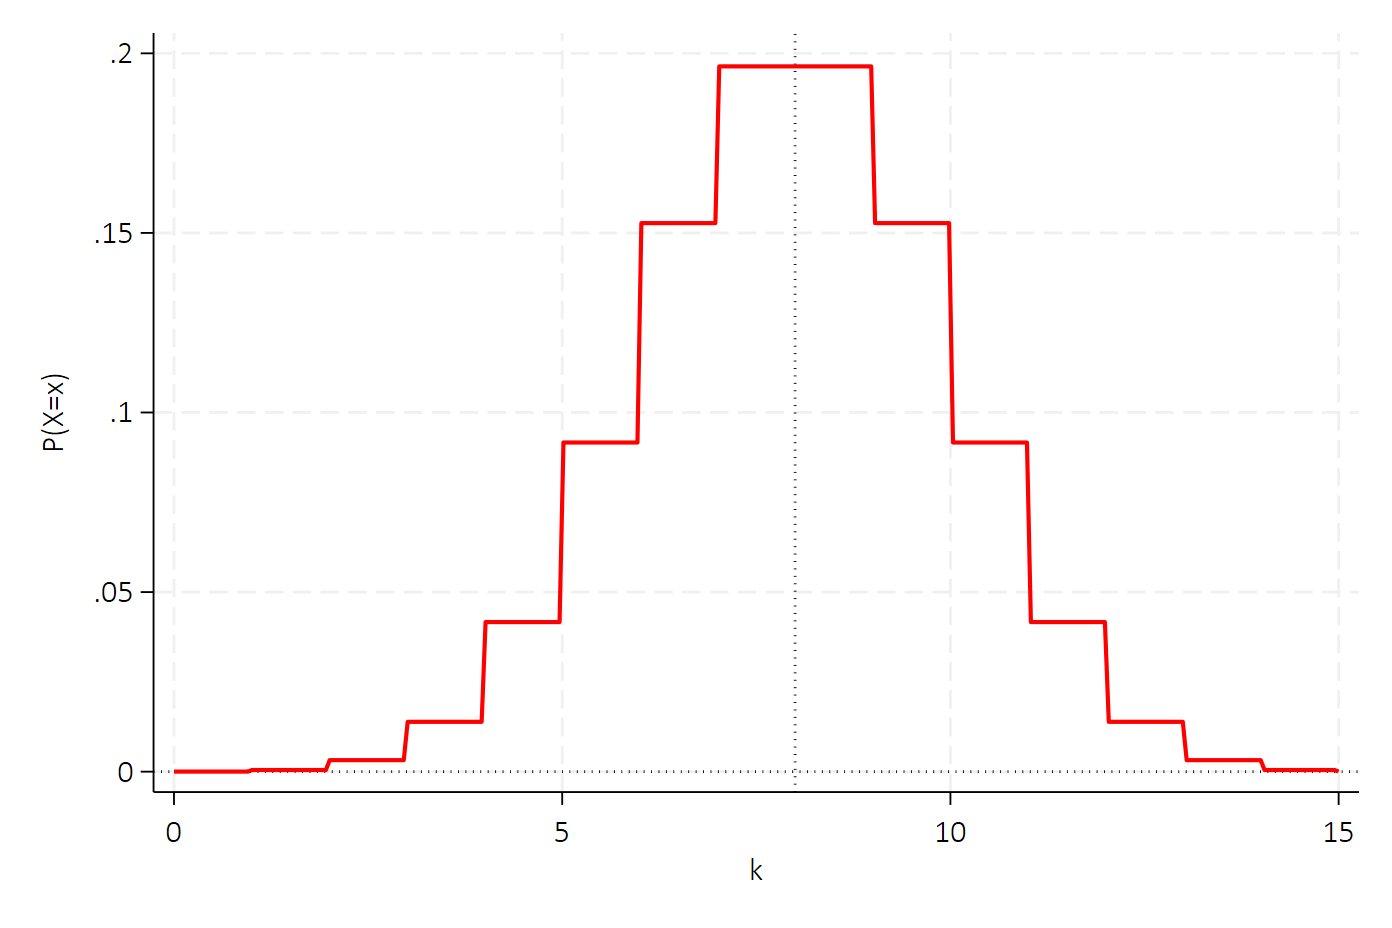
\includegraphics[width=0.45\textwidth]{figures/binomial_pdf}
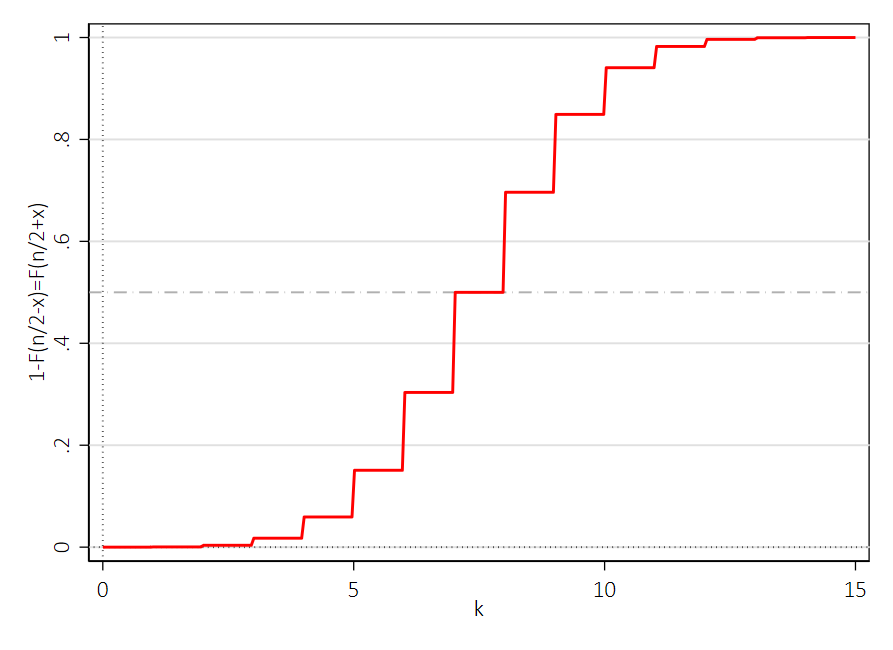
\includegraphics[width=0.45\textwidth]{figures/binomial_cdf}}\label{f2}
\end{center}
\end{figure}
\end{frame}


\begin{frame}{Discrete distributions}

The limiting form of the binomial distribution, $n\rightarrow\infty$, is the $\textbf{Poisson distribution}$,
\begin{equation*}
    Prob(X = x) =\frac{e^{\lambda}\lambda^{x}}{x!}.
\end{equation*}
The mean and variance of $x$ are
\begin{itemize}
	\item  $E[x]=\lambda$ and 
	\item $V[x]=\lambda$.
\end{itemize}

Example of a Poisson $[3]$ distribution:

\begin{figure}[H]
\begin{center}
%\scalebox{.36}
{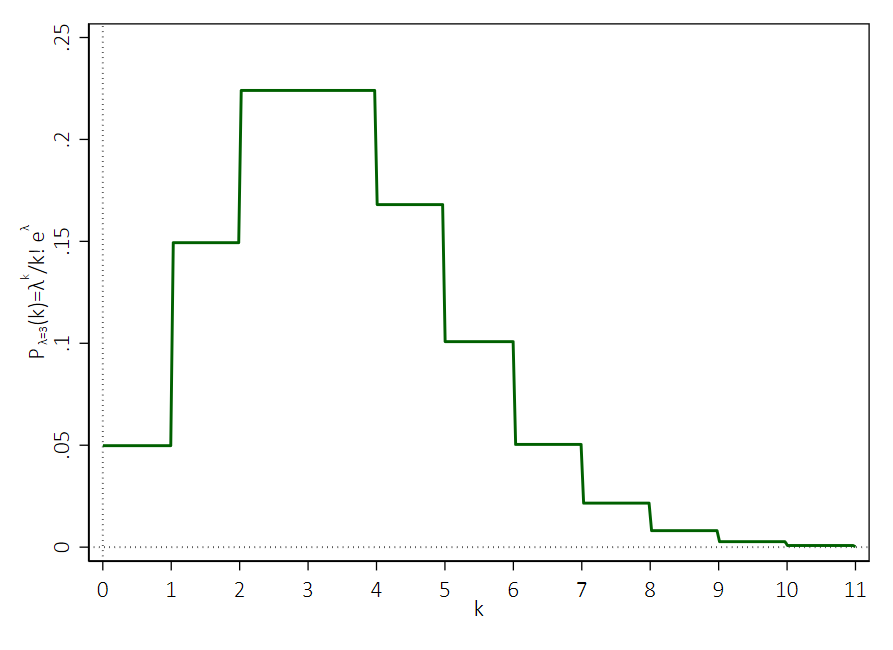
\includegraphics[width=0.45\textwidth]{figures/poisson_pdf}}\label{f4}
\end{center}
\end{figure}
\end{frame}




\section{The normal distribution}

\begin{frame}{The normal distribution}

Random variable $x \sim N[\mu, \sigma^{2}]$ is distributed according to the $\textbf{normal distribution}$ with mean $\mu$ and standard deviation $\sigma$ obtained as
\begin{equation}
    f(x|\mu, \sigma)=\frac{1}{\sigma\sqrt{2\pi}}e^{-\frac{1}{2}(\frac{x-\mu}{\sigma})^2}.
\end{equation}

The density is denoted $\phi(x)$ and the cumulative distribution function is denoted $\Phi(x)$ for the standard normal. Example of a standard normal, ($x\sim N[0, 1]$), and a normal with mean $0.5$ and standard deviation $1.3$:

\begin{figure}[H]
\begin{center}
%\scalebox{.36}
{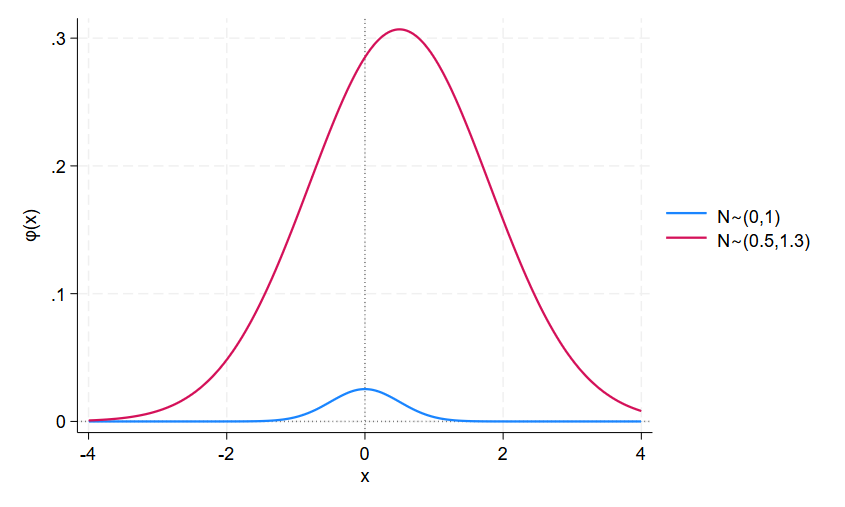
\includegraphics[width=0.45\textwidth]{figures/normals_pdf}}\label{f4}
\end{center}
\end{figure}
\end{frame}


\section{Method of transformations}
\begin{frame}{Transformation of random variables}
\renewcommand{\baselinestretch}{1.45}

Continuous variable $x$ may be transformed to a discrete variable $y$. Calculate the mean of variable $x$ in the respective interval:
\begin{eqnarray*}
  Prob(Y = \mu_{1}) &=& P(-\infty < X \leq a), \\
  Prob(Y = \mu_{2})  &=& P(a < X \leq b), \\
  Prob(Y = \mu_{3})  &=& P(b < X \leq \infty).\\
\end{eqnarray*}

\end{frame}


\begin{frame}{Method of transformations}
\renewcommand{\baselinestretch}{1.}
\scriptsize
If $x$ is a continuous random variable with pdf $f_{x}(x)$ and if $y = g(x)$ is a continuous monotonic function of $x$, then the density of $y$ is obtained by
\begin{equation*}
    Prob(y \leq b) =\int_{-\infty}^{b}f_{x}(g^{-1}(y))|g^{-1\prime}(y)|dy.
\end{equation*}
With $f_{y}(y)=f_{x}(g^{-1}(y))|g^{-1\prime}](y)|dy$, this equation can be written as
$$Prob(y \leq b) =\int_{-\infty}^{b}f_{y}(y)dy.$$
\begin{example}\renewcommand{\baselinestretch}{0.9}
\scriptsize
If $x \sim N[\mu, \sigma^{2}],$ then the distribution of $y=g(x)=\frac{x-\mu}{\sigma}$ is found as follows:
$$g^{-1}(y)= x=\sigma y+\mu$$
$$g^{-1\prime}(y)= \frac{dx}{dy}=\sigma$$
Therefore with $f_x(x)=\frac{1}{\sigma\sqrt{2\pi}}e^{-\frac{1}{2}[(g^{-1}(y)-\mu)^2/\sigma^{2}]}|g^{-1\prime}(y)|$
\begin{equation*}
    f_{y}(y)=\frac{1}{\sqrt{2\pi}\sigma}e^{-[(\sigma y+\mu)-\mu]^{2}/2\sigma^{2}}|\sigma|=\frac{1}{\sqrt{2\pi}}e^{-y^{2}/2}.
\end{equation*}
\end{example}

\end{frame}

\begin{frame}{Properties of the normal distribution}
\renewcommand{\baselinestretch}{1.45}

\begin{itemize}
	\item Preservation under linear transformation:\\
 If $x \sim N[\mu, \sigma^{2}],$ then $(a + bx) \sim N[a + b\mu, b^{2}\sigma^{2}].$
\item Convenient transformation $a = -\mu/\sigma$ and $b = 1/\sigma$:\\
 The resulting variable $z=\frac{(x - \mu)}{\sigma}$ has the standard normal distribution with density $$\phi(z)=\frac{1}{\sqrt{2\pi}}e^{-\frac{z^{2}}{2}}.$$
\item If $x \sim N[\mu,\sigma^{2}]$, then $f(x)=\frac{1}{\sigma}\phi[\frac{x-\mu}{\sigma}]$
\item $Prob(a \leq x \leq b) = Prob\left(\frac{a-\mu}{\sigma}\leq\frac{x-\mu}{\sigma}\leq\frac{b-\mu}{\sigma}\right)$
\item $\phi(-z) = 1 - \phi(z)$ and $\Phi(-x)=1-\Phi(x)$ because of symmetry
\end{itemize}
\end{frame}


\begin{frame}{Method of transformations}
\renewcommand{\baselinestretch}{1.}
If $z \sim N[0, 1]$, then $z^{2} \sim \chi^2[1]$ with pdf $\frac{1}{\sqrt{2\pi y}}e^{-y/2}$.
\begin{example}\renewcommand{\baselinestretch}{0.9}
\scriptsize
$$f_x(x)=\frac{1}{\sqrt{2\pi}}e^{-\frac{x^2}{2}}$$
$$y=g(x)=x^2$$
$$g^{-1}(y)= x=\pm \sqrt{y} \text{ there are two solutions to } g_1,g_2.$$
$$g^{-1\prime}(y)= \frac{dx}{dy}=\pm 1/2y^{-1/2}$$
$$f_{y}(y)=f_x(g_1^{-1}(y))|g_1^{-1\prime}(y)|+f_x(g_2^{-1}(y))|g_2^{-1\prime}(y)|$$
$$f_{y}(y)=f_x(\sqrt{y})|1/2y^{-1/2}|+f_x(-\sqrt{y})|-1/2y^{-1/2}|$$
$$f_{y}(y)=\frac{1}{2\sqrt{2\pi y}}e^{-\frac{y}{2}}+\frac{1}{2\sqrt{2\pi y}}e^{-\frac{y}{2}}=\frac{1}{\sqrt{2\pi y}}e^{-\frac{y}{2}}$$
\end{example}

\end{frame}

\begin{frame}{Distributions derived from the normal}
\footnotesize
\begin{itemize}
  \item If $z \sim N[0, 1]$, then $z^{2} \sim \chi^2[1]$ with $E[z^2]=1$ and $V[z^2]=2$.
  \item If $x_{1},..., x_{n}$ are $n$ independent $\chi^2[1]$ variables, then $$\sum_{i=1}^{n}x_{i}\sim \chi^2[n].$$
  \item If $z_{i},i = 1,..., n,$ are independent $N[0, 1]$ variables, then $$\sum_{i=1}^{n}z_{i}^{2}\sim \chi^{2}[n].$$
  \item If $z_{i},i = 1,..., n$, are independent $N[0, \sigma^2]$ variables, then $$\sum_{i=1}^{n}\bigg(\frac{z_{i}}{\sigma}\bigg)^{2}\sim \chi^{2}[n].$$
  \item If $x_{1}$ and $x_{2}$ are independent $\chi^2$ variables with $n_{1}$ and $n_{2}$ degrees of freedom, then $$x_{1} + x_{2} \sim \chi^{2}[n_{1} + n_{2}].$$
\end{itemize}
\end{frame}


\section{The $\chi^2$ distribution}
\begin{frame}{The $\chi^2$ distribution}

Random variable $x \sim \chi^2[n]$ is distributed according to the $\textbf{ chi-squared distribution}$ with $n$ degrees of freedom
\begin{equation}
    f(x|n)=\dfrac{x^{n/2 -1} e^{-x/2}}{2^{n/2} \Gamma\left(\frac n 2 \right)},
\end{equation}

where $\Gamma$ is the Gamma-distribution (more below).
\begin{itemize}
	\item $E[x]=n$
  \item $V[x]=2n$
\end{itemize}
Example of a $\chi^2[3]$ distribution:

\begin{figure}[H]
\begin{center}
%\scalebox{.36}
{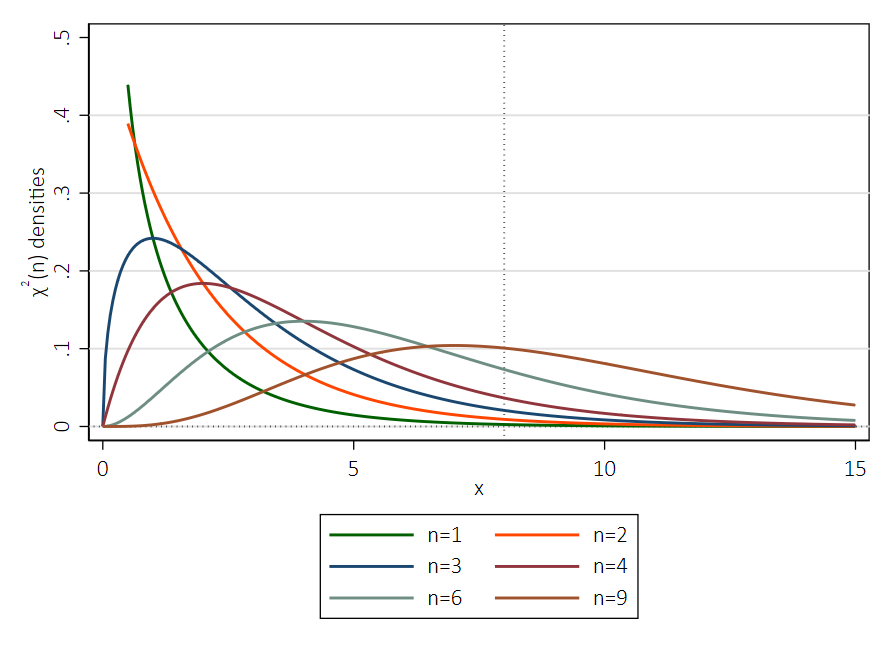
\includegraphics[width=0.45\textwidth]{figures/chi2_pdf}
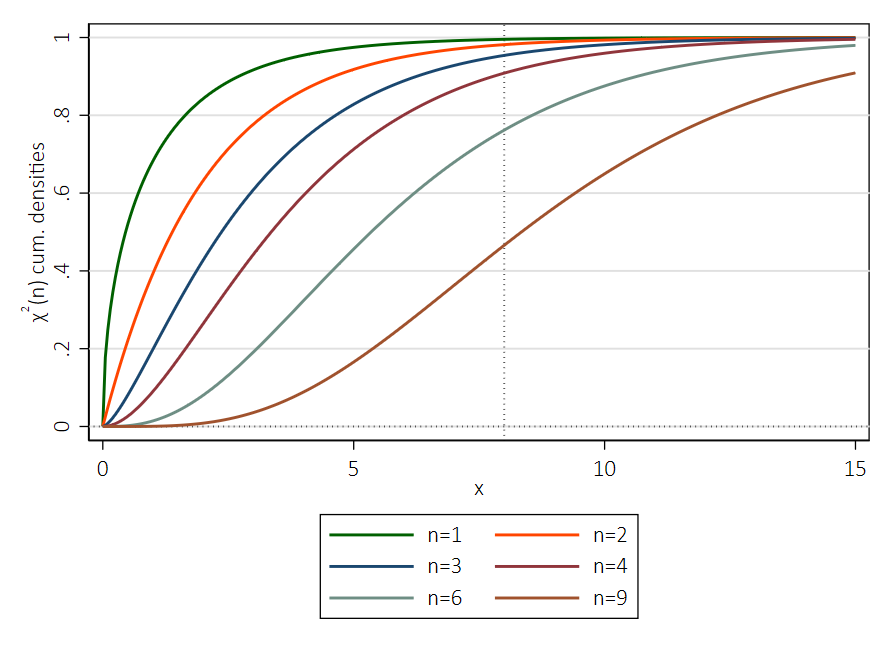
\includegraphics[width=0.45\textwidth]{figures/chi2_cdf}}\label{f2}\end{center}
\end{figure}
\end{frame}



\section{The F-distribution}
\begin{frame}{The F-distribution}
If $x_{1}$ and $x_{2}$ are two independent chi-squared variables with degrees of freedom parameters
   $n_{1}$ and $n_{2}$, respectively, then the ratio
   \begin{equation}\label{eq11}
    F [n_{1}, n_{2}] = \frac{x_{1}/n_{1}}{x_{2}/n_{2}}
   \end{equation}
   has the $\textbf{F distribution}$ with $n_{1}$ and $n_{2}$ degrees of freedom.

\begin{figure}[H]
\begin{center}
%\scalebox{.36}
{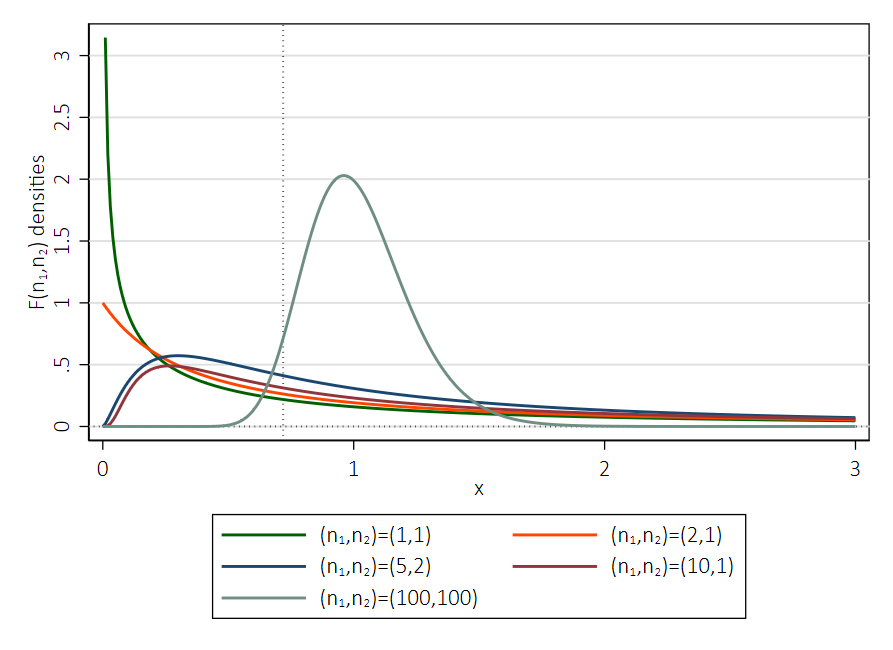
\includegraphics[width=0.45\textwidth]{figures/F_pdf}
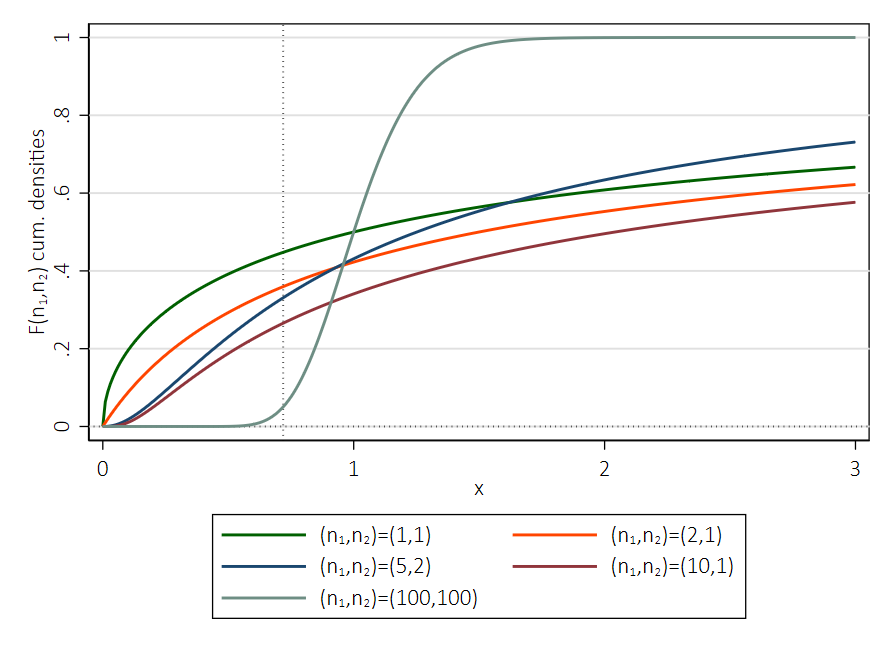
\includegraphics[width=0.45\textwidth]{figures/F_cdf}}\label{f3}
\end{center}
\end{figure}

\end{frame}



\section{The student t-distribution}
\begin{frame}{The student t-distribution}
If $z$ is an $N[0, 1]$ variable and $x$ is $\chi^{2}[n]$ and is independent of $z$, then the ratio
  \begin{equation}\label{eq12}
    t[n] = \frac{z}{\sqrt{x/n}}.
  \end{equation}
  has the $\textbf{t distribution}$ with $n$ degrees of freedom.
 
Example for the $t$ distributions with $3$ and $10$ degrees of freedom with the standard normal distribution.
\begin{figure}[H]
\begin{center}
%\scalebox{.36}
{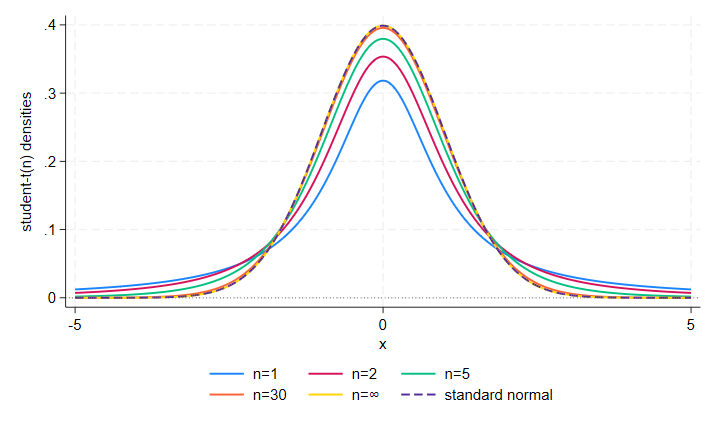
\includegraphics[width=0.45\textwidth]{figures/t_pdf}
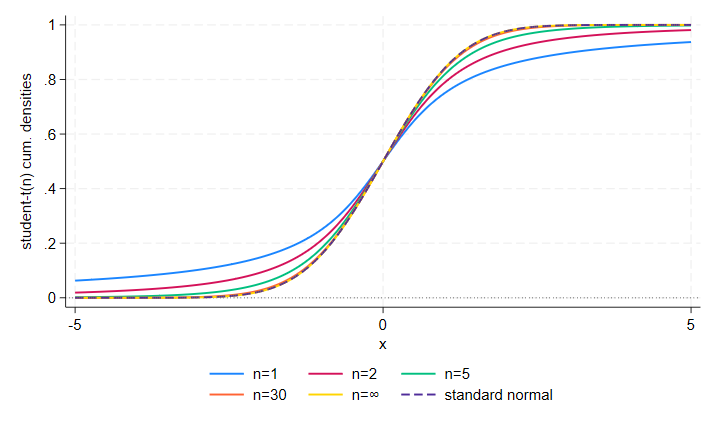
\includegraphics[width=0.45\textwidth]{figures/t_cdf}}\label{f3}
\end{center}
\end{figure}

Comparing (\ref{eq11}) with $n_{1} = 1$ and (\ref{eq12}), if $t \sim t[n]$, then $t^{2} \sim F[1, n]$.

\end{frame}


\begin{frame}{The $t[30]$ approx. the standard normal}

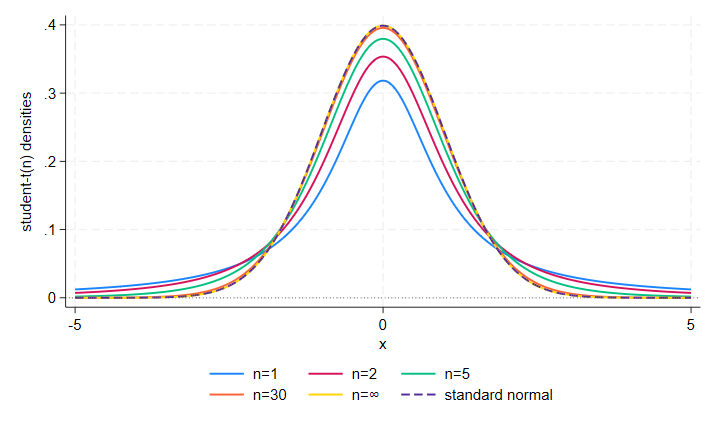
\includegraphics[width=0.9\textwidth]{figures/t_pdf}
\end{frame}

\begin{frame}{Approximating a $\chi^2$}
For degrees of freedom greater than $30$ the distribution of the chi-squared variable $x$ is approx.
\begin{equation}\label{eq13}
    z = (2x)^{1/2} - (2n - 1)^{1/2},
\end{equation}
which is approximately standard normally distributed. Thus,
\begin{equation*}
    Prob(\chi^{2}[n] \leq a) \approx \Phi[(2a)^{1/2} - (2n - 1)^{1/2}].
\end{equation*}

\begin{figure}[H]
\begin{center}
%\scalebox{.36}
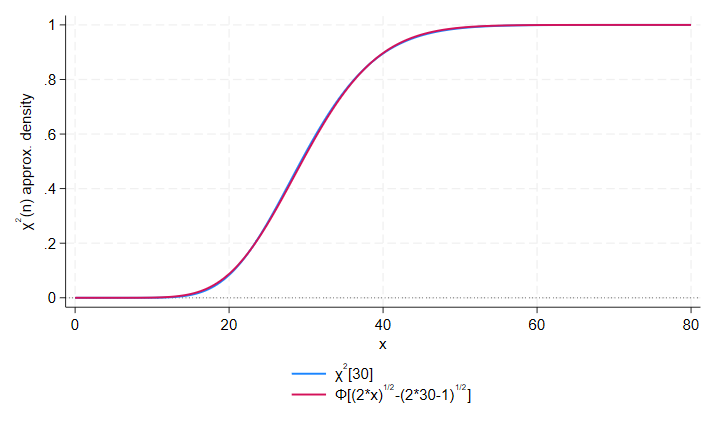
\includegraphics[width=0.6\textwidth]{figures/chi2_cdf_approx
}\label{ch1}
\end{center}
\end{figure}

\end{frame}




\section{The lognormal distribution}
\begin{frame}{The lognormal distribution}
The $\textbf{lognormal distribution}$, denoted $LN[\mu,\sigma^{2}]$, has been particularly
useful in modeling the size distributions.
\begin{equation*}
    f(x) = \frac{1}{\sqrt{2\pi}\sigma x}e^{-\frac{1}{2[(\ln x-\mu)/\sigma]^{2}}},~~~~~~~x>0
\end{equation*}
A lognormal variable $x$ has
\begin{itemize}
	\item  $E[x]= e^{\mu+\sigma^{2}/2},$ and
	\item $Var[x]= e^{2\mu+\sigma^{2}}(e^{\sigma^{2}}-1).$
\end{itemize}

If $y \sim LN[\mu,\sigma^{2}],$ then $\ln y \sim N[\mu,\sigma^{2}].$
\begin{figure}[H]
\begin{center}
%\scalebox{.36}
{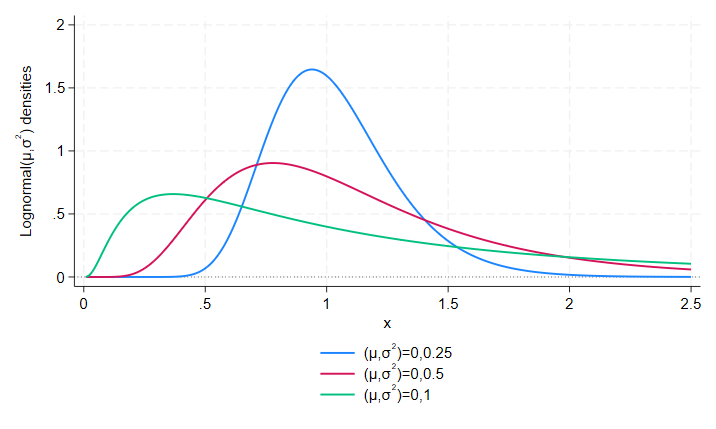
\includegraphics[width=0.45\textwidth]{figures/lnnormal_pdf}
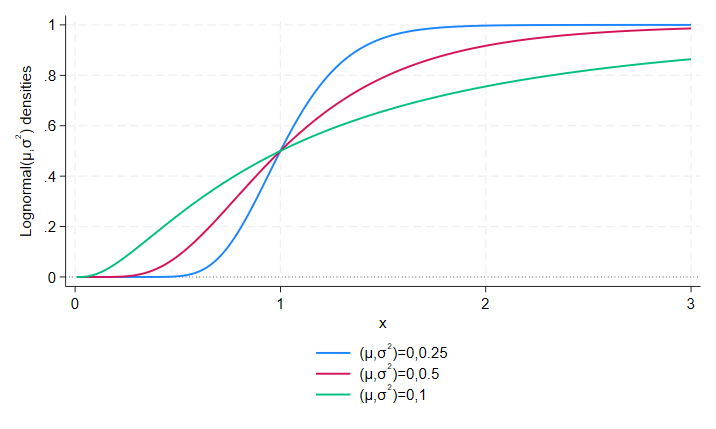
\includegraphics[width=0.45\textwidth]{figures/lnnormal_cdf}}\label{f2}
\end{center}
\end{figure}
\end{frame}


\section{The gamma distribution}
\begin{frame}{The gamma distribution}
The general form of the $\textbf{gamma distribution}$ is
\begin{equation}
    f(x) = \frac{\lambda^{P}}{\Gamma (P)}e^{-\lambda x}x^{P-1},~~~~~~~x\geq0, \lambda>0, P>0.
\end{equation}
Many familiar distributions are special cases, including the $\textbf{exponential distribution} (P = 1)$ and
$\textbf{chi-squared} (\lambda = 1/2 , P = n/2 )$. The $\textbf{Erlang distribution}$ results if $P$ is a positive integer. The mean is
$P/\lambda$, and the variance is $P/\lambda^{2}$. The $\textbf{inverse gamma distribution}$ is the distribution of $1/x$, where $x$ has the gamma distribution.
\begin{figure}[H]
\begin{center}
%\scalebox{.36}
{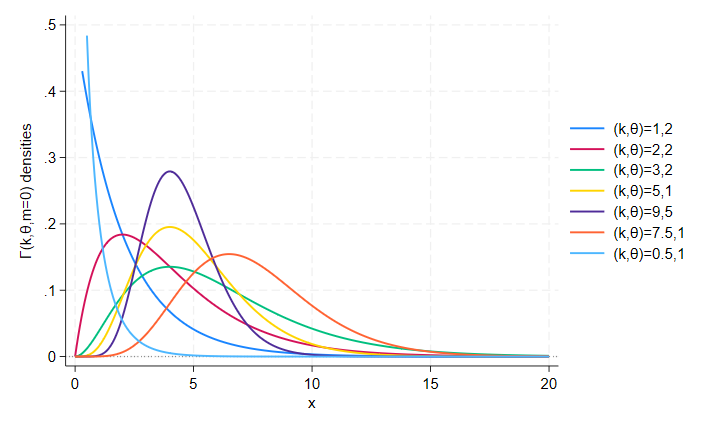
\includegraphics[width=0.45\textwidth]{figures/gamma_pdf}
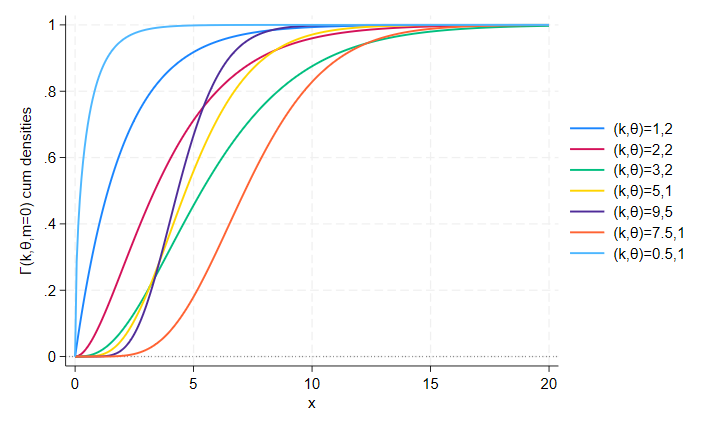
\includegraphics[width=0.45\textwidth]{figures/gamma_cdf}}\label{f2}
\end{center}
\end{figure}
\end{frame}


\section{The beta distribution}
\begin{frame}{The beta distribution}
For a variable constrained between $0$ and $c > 0$, the $\textbf{beta distribution}$ has proved useful. Its density is
\begin{equation*}
    f(x) = \frac{\Gamma(\alpha+\beta)}{\Gamma (\alpha)\Gamma(\beta)}\left(\frac{x}{c}\right)^{\alpha-1}\left(1-\frac{x}{c}\right)^{\beta-1}\frac{1}{c},~~~~~~~x\geq0, \lambda>0, P>0.
\end{equation*}
It is symmetric if $\alpha = \beta$, asymmetric otherwise.  The mean is $ca/(\alpha + \beta)$,
and the variance is $c^{2}\alpha\beta/[(\alpha +\beta +1)(\alpha +\beta)^{2}]$.
\begin{figure}[H]
\begin{center}
{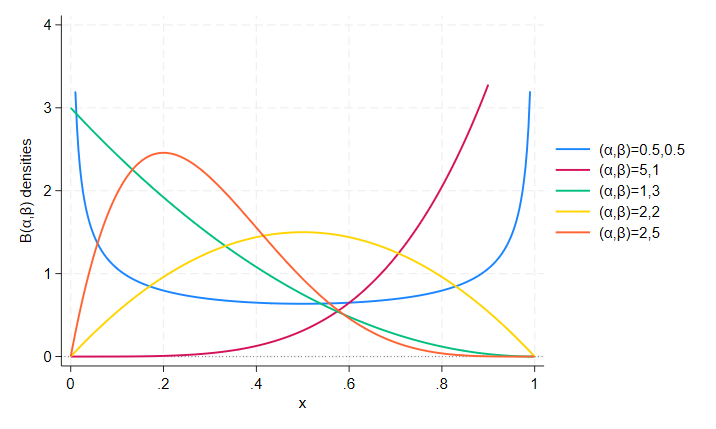
\includegraphics[width=0.45\textwidth]{figures/beta_pdf}
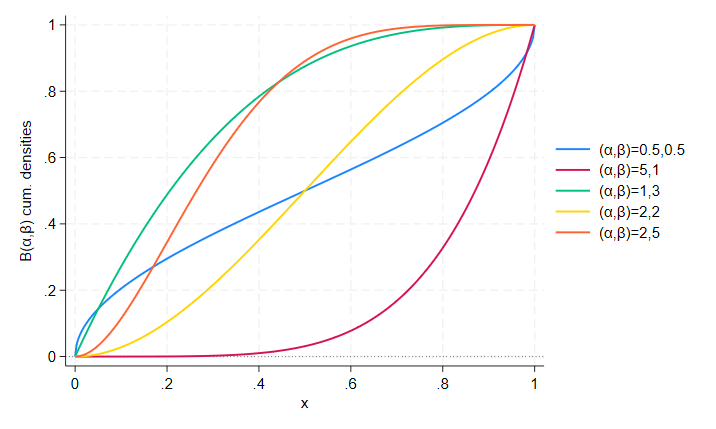
\includegraphics[width=0.45\textwidth]{figures/beta_cdf}}\label{f2}
\end{center}
\end{figure}
\end{frame}


\section{The logistic distribution}
\begin{frame}{The logistic distribution}
The $\textbf{logistic distribution}$ is an alternative if the normal cannot model the mass in the tails; the cdf for a logistic random variable is
\begin{equation*}
    F(x) =\Lambda(x)= \frac{1}{1+e^{-x}}.
\end{equation*}
The density is $f(x) = \Lambda(x)[1 - \Lambda(x)]$. The mean and variance of this random variable are zero
and $\pi^{2}/3$.
\begin{figure}[H]
\begin{center}
{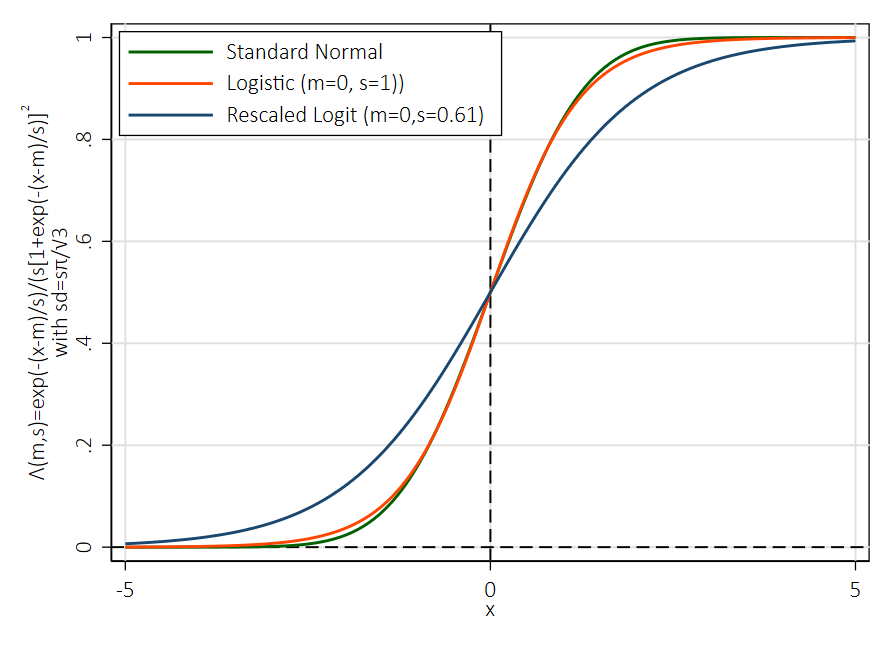
\includegraphics[width=0.5\textwidth]{figures/normal_logistic_cdf}}\label{f2}
\end{center}
\end{figure}
\end{frame}



\section{The Wishart distribution}
\begin{frame}{The Wishart distribution}

{ The $\textbf{Wishart distribution}$ describes the distribution of a random matrix obtained as
\begin{equation*}
    f(\bm{W}) =\sum_{i=1}^{n}(x_{i}-\mu)(x_{i}-\mu)^{\prime}.
\end{equation*}
where $x_{i}$ is the $i$th of $n K$ element random vectors from the multivariate normal distribution with
mean vector, $\mu$, and covariance matrix, $\Sigma$.  The density of the Wishart random matrix is
\begin{equation*}
    f(\bm{W}) =\frac{\exp\left[-\frac{1}{2}trace(\Sigma^{-1}\bm{W})\right]|\bm{W}|^{-\frac{1}{2}(n-K-1)}}{2^{nK/2}|\Sigma|^{K/2}\pi^{K(K-1)/4}\prod_{j=1}^{K}\Gamma\left(\frac{n+1-j}{2}\right)}.
\end{equation*}
The mean matrix is $n\Sigma$. For the individual pairs of elements in $\bm{W}$,
\begin{equation*}
    Cov[w_{ij}, w_{rs}] = n(\sigma_{ir}\sigma_{js} + \sigma_{is}\sigma_{jr}).
\end{equation*}}
The Wishart distribution is a multivariate extension of $\chi^2$ distribution. If $\bm{W}\sim W(n,\sigma^2)$, then $\bm{W}/\sigma^2\sim\chi^2[n].$
\end{frame}


\begin{frame}[t,allowframebreaks
]\nocite{*}
\frametitle{References}
\small
\bibliography{bib}
\end{frame}


\end{document}
